\appendix
\clearpage
\raggedcolsend
\raggedend
\raggedbottom

\setlength{\textfloatsep}{6pt plus 2pt minus 1pt}
\setlength{\floatsep}{4pt plus 2pt minus 1pt}
\setlength{\intextsep}{7pt plus 2pt minus 1pt}
\setlength{\dbltextfloatsep}{7pt plus 2pt minus 1pt}
\setlength{\dblfloatsep}{5pt plus 2pt minus 1pt}
\makeatletter
\setlength{\@dblfptop}{0pt}
\setlength{\@dblfpsep}{10pt}
\setlength{\@dblfpbot}{0pt plus 1fil}
\makeatother

\section{Intervention Details}
\label{app:method}

\paragraph{Attention-diagonal editing.}
Equation~\ref{eq:general-diagonal-constraint} defines the requested change in
the parallel component. Let $\mathbf m_t$ be the self message,
$\mathbf r_t$ the reference, and $\mathcal B_{tt}$ its linear map into the
edited space. One minimum-Frobenius-norm realization of
$\Delta\mathbf y_{tt}=\Delta\mathcal B_{tt}\mathbf m_t$ is
\[
  \Delta\mathcal{B}_{tt}^{\star}
  =
  \bigl(s^{(\parallel)}-1\bigr)
  \frac{\mathbf{y}_t^\top\mathbf{r}_t}
       {\|\mathbf{m}_t\|^2\|\mathbf{r}_t\|^2}
  \mathbf{r}_t\mathbf{m}_t^\top.
\]
For a structured operator family, the same construction uses the Frobenius
projection of \(\mathbf{r}_t\mathbf{m}_t^\top\) onto the admissible operator
subspace.
Table~\ref{tab:effective-diagonal-derivation} gives the resulting scalar forms.
For the exclude-self variant used in our primary value-space results,
Eq.~\ref{eq:exclude-self-scaling} instead applies the projection to
\(\sum_{s<t}A_{ts}\mathbf{v}_s\) and then restores the unchanged direct term
\(A_{tt}\mathbf{v}_t\).

\begin{table}[H]
  \caption{\textbf{Attention-diagonal forms for component scaling.} The value-space
  form is exact; the residual form matches only the scalar projection
  constraint. ``Removed case'' sets $s^{(\parallel)}=0$ while retaining the
  perpendicular component.}
  \label{tab:effective-diagonal-derivation}
  \centering
  \scriptsize
  \setlength{\tabcolsep}{2pt}
  \begingroup
  \renewcommand{\arraystretch}{1.12}
  \begin{tabularx}{\linewidth}{>{\raggedright\arraybackslash}p{0.28\linewidth}X}
    \toprule
    Quantity & Form \\
    \midrule
    \multicolumn{2}{c}{\textit{Full-aggregate value space}} \\
    \cmidrule(lr){1-2}
    \addlinespace[2pt]
    Diagonal change &
    \(\Delta A_{tt}=(s^{(\parallel)}-1)
      \frac{\mathbf{o}_t^\top\mathbf{v}_t}{\|\mathbf{v}_t\|^2}\). \\
    Removed case &
    \(\widetilde A_{tt}=
      -\sum_{s<t}A_{ts}
      \frac{\mathbf{v}_s^\top\mathbf{v}_t}{\|\mathbf{v}_t\|^2}\). \\
    \midrule
    \multicolumn{2}{c}{\textit{Residual space}} \\
    \cmidrule(lr){1-2}
    \addlinespace[2pt]
    Diagonal change &
    \(\Delta A_{tt}=(s^{(\parallel)}-1)
      \frac{(\Delta_t^{\Attn})^\top\hz{}{t}}
           {(W_O\mathbf{v}_t)^\top\hz{}{t}}\). \\
    Removed case &
    \(\widetilde A_{tt}=A_{tt}
      -\sum_{s\le t}A_{ts}
      \frac{(W_O\mathbf{v}_s)^\top\hz{}{t}}
           {(W_O\mathbf{v}_t)^\top\hz{}{t}}\). \\
    \bottomrule
  \end{tabularx}
  \endgroup
\end{table}


\paragraph{Applied strength of the two edits.}
Table~\ref{tab:applied-no-para-strength} audits both Full No-Para edits at a
common post-$W_O$ site. The exclude-self value-space edit applies the larger
perturbation on every measure, so its smaller behavioral cost does not follow
from a gentler intervention.
\begin{table}[H]
  \centering
  \footnotesize
  \caption{\textbf{Applied strength of attention Full No-Para interventions.}
  Full No-Para sets $s_{\parallel}=0$. Ratios are measured at the summed
  attention output on Qwen3-0.6B; value-space
  attention preserves the self term and is mapped through $W_O$. Perturbation
  and retained norm compare $\|\widetilde y-y\|$ and $\|\widetilde y\|$ with
  $\|y\|$; energy is the sample average of $\|\widetilde y-y\|^2/\|y\|^2$.}
  \label{tab:applied-no-para-strength}
  \begingroup
  \renewcommand{\arraystretch}{1.32}
  \setlength{\tabcolsep}{2pt}
  \resizebox{\columnwidth}{!}{%
  \begin{tabular}{lrrr}
    \toprule
    Geometry & \shortstack{Perturbation\\norm}
             & \shortstack{Perturbation\\energy}
             & \shortstack{Retained\\norm} \\
    \midrule
    Attention residual-space & 25.15\% & 9.323\% & 95.01\% \\
    Attention exclude-self value-space & 49.10\% & 25.89\% & 83.36\% \\
    \bottomrule
  \end{tabular}
  }
  \endgroup
\end{table}

\paragraph{Forward-hook implementation.}
We apply Eq.~\ref{eq:unified-component-scaling} through forward hooks that
replace only the selected tensor; all subsequent computation is unchanged.
Table~\ref{tab:projection-overhead} reports the measured cost.

\begin{table}[H]
  \centering
  \scriptsize
  \setlength{\tabcolsep}{3pt}
  \caption{\textbf{Measured pre-\(W_O\) projection overhead.}
  Wall-clock increases relative to the unedited baseline are measured on one
  RTX 6000 Ada. BF16 inference uses batch 2: prefill has length 2,048 and decode
  generates one token from a 512-token static cache with CUDA Graph replay.
  Training uses the 0.7B model with batch 1 and length 2,048. The three
  inference values are ordered as Qwen3-0.6B/4B/14B.}
  \label{tab:projection-overhead}
  \begin{tabular}{lc}
    \toprule
    Workload & Optimized overhead \\
    \midrule
    Prefill
      & 2.47\% / 1.25\% / 1.11\% \\
    Static graph decode
      & 0.83\% / 0.36\% / 0.25\% \\
    Training (0.7B)
      & 3.39\% \\
    \bottomrule
  \end{tabular}
\end{table}

The fused kernel combines the dot product, norm, and projection update with
FlashAttention-2~\citep{dao2024flashattention2}.

\section{Evaluation Details}
\label{app:evaluation-details}

\paragraph{Evaluated models.}
The editing and diagnostic experiments use Qwen3~\citep{Yang2025Qwen3TR}, and
individual figures and tables name the evaluated scale. Qwen3-4B results use
the base checkpoint, except Figure~\ref{fig:profiles}, which uses
Qwen3-4B-Instruct-2507. Long-context evaluation uses
Llama-3.2-3B~\citep{Dubey2024TheL3}.

\paragraph{Benchmark evaluation.}
Benchmark and RULER tasks are executed through the Language Model Evaluation
Harness~\citep{eval-harness}. RULER~\citep{Hsieh2024RULERWT} provides the
long-context evaluation. Task definitions follow the original sources for
CoQA~\citep{reddy-etal-2019-coqa}, DROP~\citep{dua-etal-2019-drop},
TruthfulQA~\citep{lin-etal-2022-truthfulqa}, and the remaining
benchmarks~\citep{Clark2018ThinkYH,
Clark2019BoolQET,Zellers2019HellaSwagCA,
Mihaylov2018CanAS,Bisk2019PIQARA,Wang2018GLUEAM,Sakaguchi2019AnAW,
Hendrycks2020MeasuringMM,Cobbe2021TrainingVT}.
Table~\ref{tab:evaluation-task-settings} gives the
default few-shot setting and metric for each task.

\clearpage
\begin{table}[H]
  \centering
  \scriptsize
  \setlength{\tabcolsep}{4pt}
  \caption{\textbf{Default evaluation task settings.} Acc. denotes accuracy;
  Norm denotes length normalization.}
  \label{tab:evaluation-task-settings}
  \begin{tabular}{@{}lcl@{}}
    \toprule
    Task & Few-shot & Metric \\
    \midrule
    ARC-Challenge & 25 & Acc. (Norm) \\
    ARC-Easy & 0 & Acc. (Norm) \\
    BoolQ & 0 & Acc. \\
    CoQA & 0 & F1 \\
    DROP & 0 & F1 \\
    GSM8K & 5 & Exact match \\
    HellaSwag & 10 & Acc. (Norm) \\
    MMLU & 5 & Acc. \\
    OpenBookQA & 0 & Acc. (Norm) \\
    PIQA & 0 & Acc. (Norm) \\
    RTE & 0 & Acc. \\
    TruthfulQA-MC1/2 & 0 & Acc. \\
    TruthfulQA generation & 0 & Rouge-L \\
    WinoGrande & 5 & Acc. \\
    \bottomrule
  \end{tabular}
  \normalsize
\end{table}

\section{Additional Editing Results}
\label{app:additional-editing}

\paragraph{Zero-shot parallel editing.}
Table~\ref{tab:appendix-ruler-full} tests whether self-preserving value-space
scaling transfers across model families on RULER-4k. At
$s_{\parallel}=0.5$, Gemma-3-12B, Llama-3.2-3B, and Qwen3-4B/8B remain within
0.5 points of their matched baselines, showing near-baseline behavior across
three model families.

\begin{table}[H]
  \centering
  \scriptsize
  \caption{\textbf{Cross-model retained-scale RULER-4k evaluation.}
  V-Excl.-self preserves the direct self contribution and sets
  $s_{\parallel}=0.5$ for the non-self aggregate; \(\Delta\) is edited minus
  matched baseline and is computed before display rounding.}
  \label{tab:appendix-ruler-full}
  \setlength{\tabcolsep}{6pt}
  \begin{tabular}{lrrr}
    \toprule
    Model & Baseline & V-Excl.-self, \(s_\parallel{=}0.5\) & \(\Delta\) \\
    \midrule
    Gemma-3-1B-IT & 68.0 & 62.8 & -5.3 \\
    Gemma-3-12B-IT & 94.0 & 94.1 & +0.1 \\
    Llama-3.2-3B & 86.9 & 86.7 & -0.2 \\
    Qwen3-0.6B & 79.8 & 75.1 & -4.8 \\
    Qwen3-1.7B & 88.1 & 84.9 & -3.2 \\
    Qwen3-4B & 92.6 & 92.4 & -0.2 \\
    Qwen3-8B & 94.2 & 93.7 & -0.5 \\
    \bottomrule
  \end{tabular}
  \normalsize
\end{table}

\paragraph{Head-level localization.}
\label{app:head-localization}
We test localization across every decoder layer of four Qwen3 scales by
comparing all isolated query-head edits with a joint all-head edit.
Figure~\ref{fig:per-head-causal-sensitivity} includes every head without
significance-based selection.

Layer 0 gives the largest positive joint effect at every scale. Beyond layer 0,
the joint effect is strongly depth-specific and often extends beyond the
corresponding single-head range.

\begin{figure*}[!t]
  \centering
  \newsavebox{\headlocalizationfigure}
  \sbox{\headlocalizationfigure}{%
    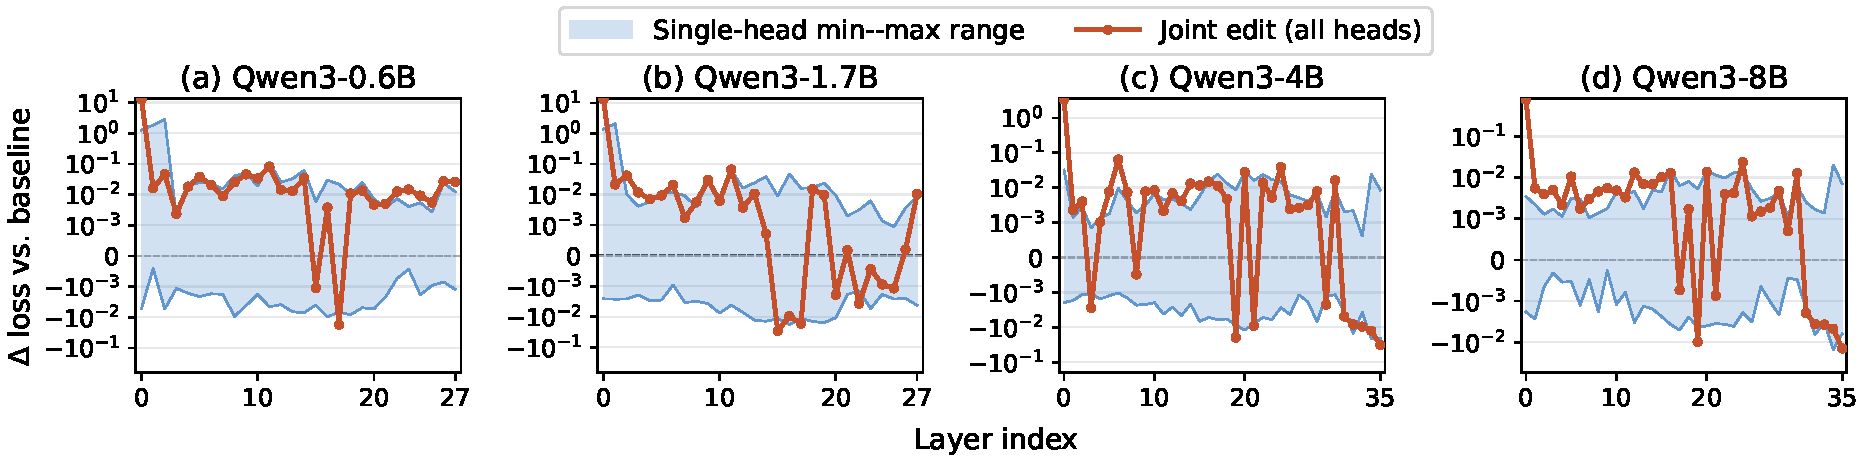
\includegraphics{figs/per_head_causal_sensitivity_fullrem/head_delta_loss.pdf}%
  }
  \ifdim\wd\headlocalizationfigure>3\ht\headlocalizationfigure
    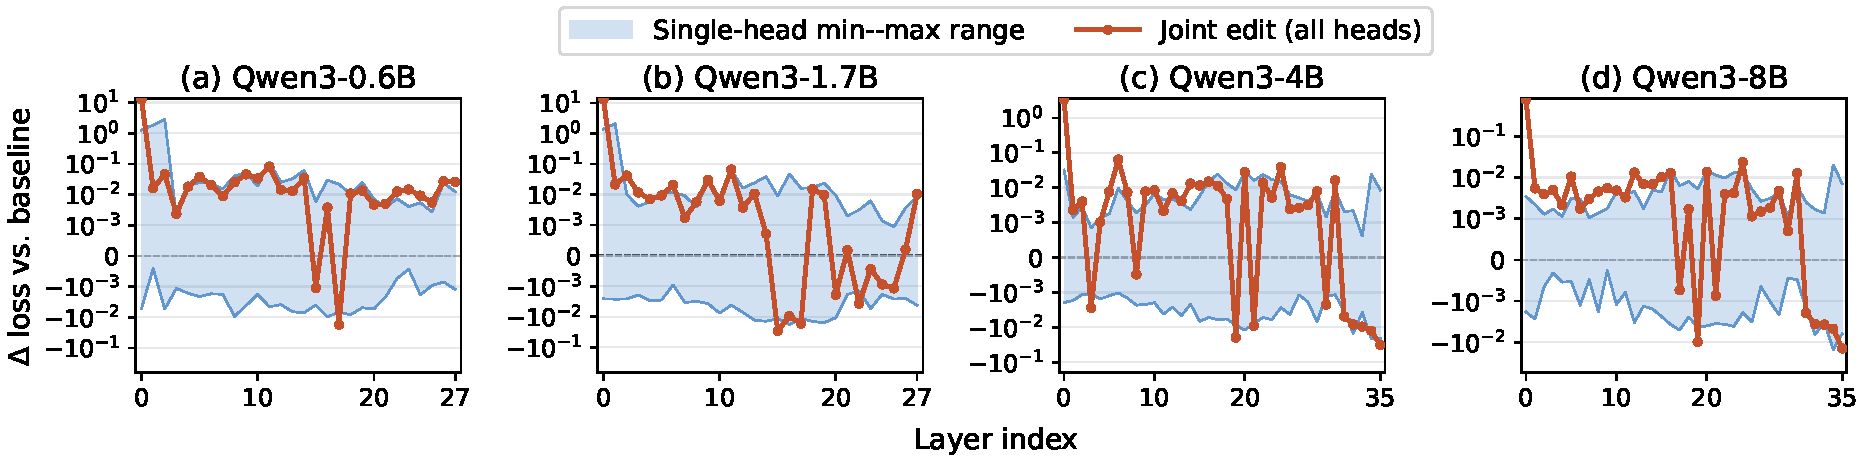
\includegraphics[width=0.98\textwidth]{figs/per_head_causal_sensitivity_fullrem/head_delta_loss.pdf}
  \else
    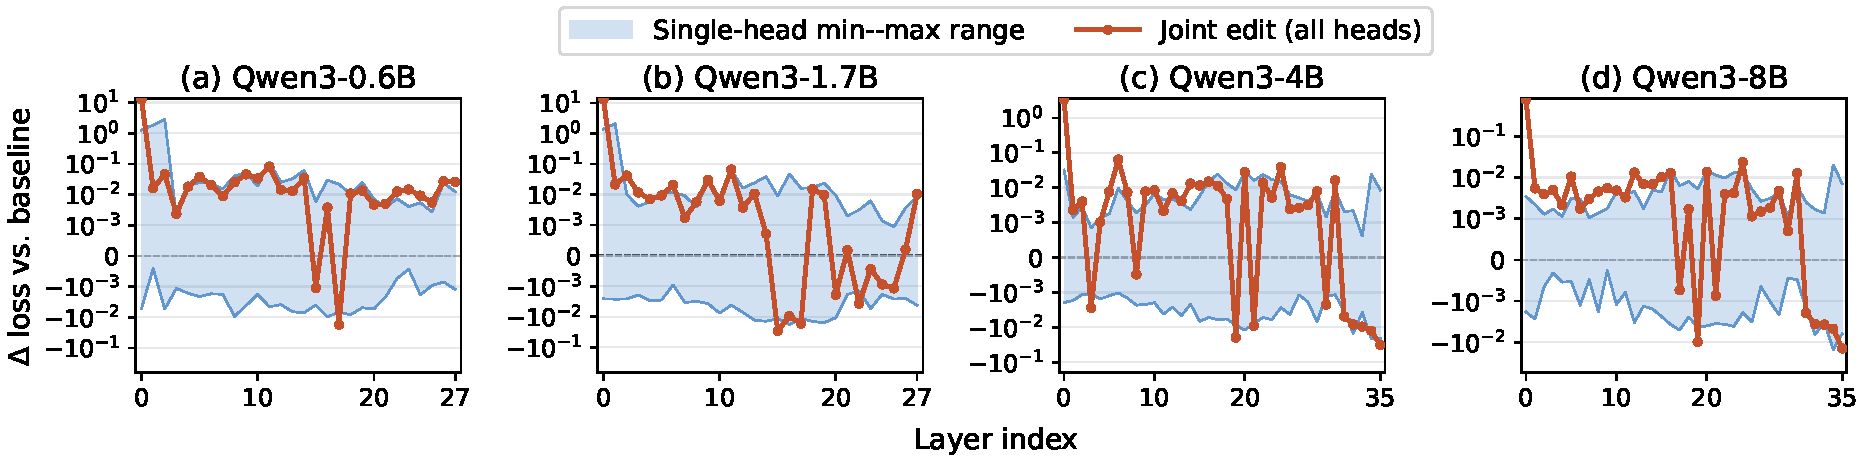
\includegraphics[
      width=0.54\textwidth,
      trim=145bp 358bp 114bp 0bp,
      clip
    ]{figs/per_head_causal_sensitivity_fullrem/head_delta_loss.pdf}

    \vspace{0.1em}
    \makebox[\textwidth][c]{%
      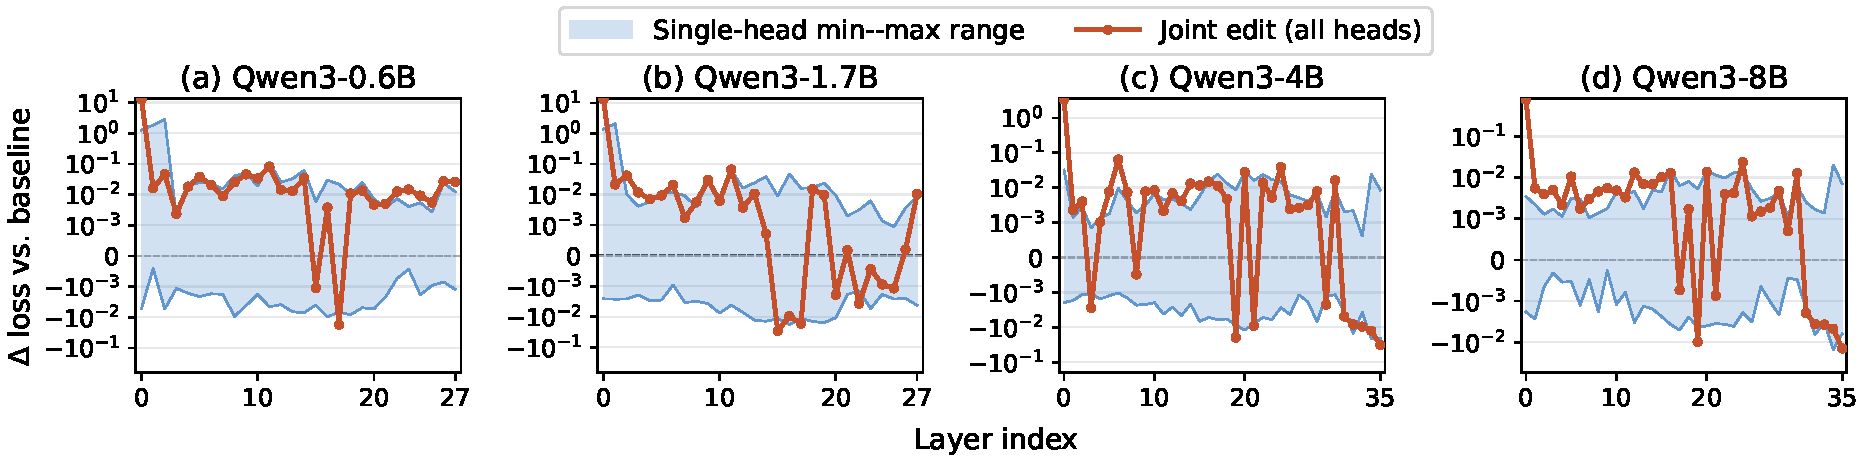
\includegraphics[
        width=0.245\textwidth,
        trim=0bp 172bp 307bp 38bp,
        clip
      ]{figs/per_head_causal_sensitivity_fullrem/head_delta_loss.pdf}%
      \hfill
      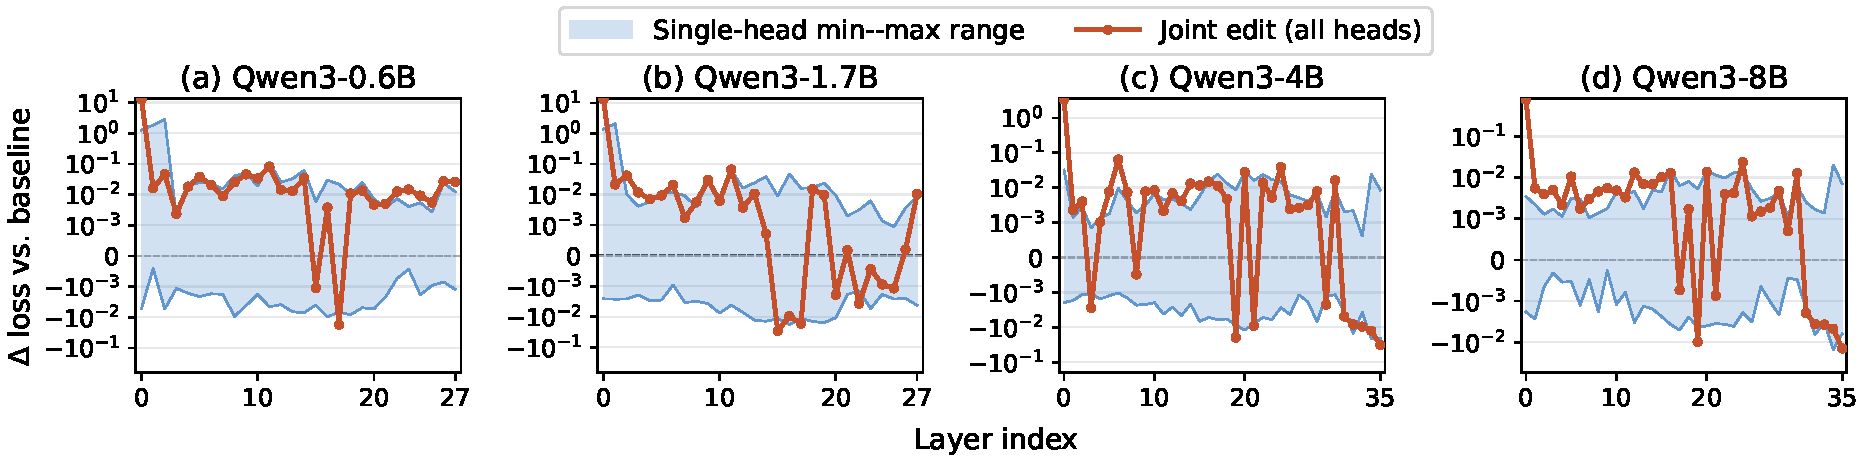
\includegraphics[
        width=0.245\textwidth,
        trim=307bp 172bp 0bp 38bp,
        clip
      ]{figs/per_head_causal_sensitivity_fullrem/head_delta_loss.pdf}%
      \hfill
      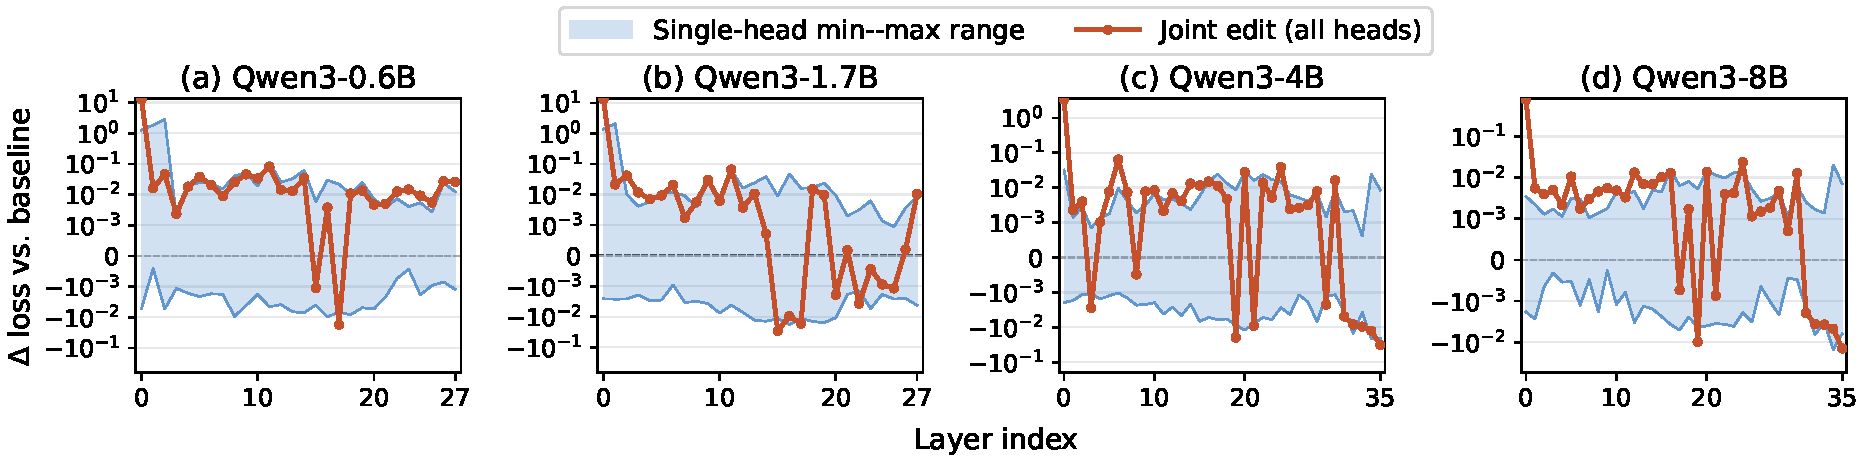
\includegraphics[
        width=0.245\textwidth,
        trim=0bp 0bp 307bp 218bp,
        clip
      ]{figs/per_head_causal_sensitivity_fullrem/head_delta_loss.pdf}%
      \hfill
      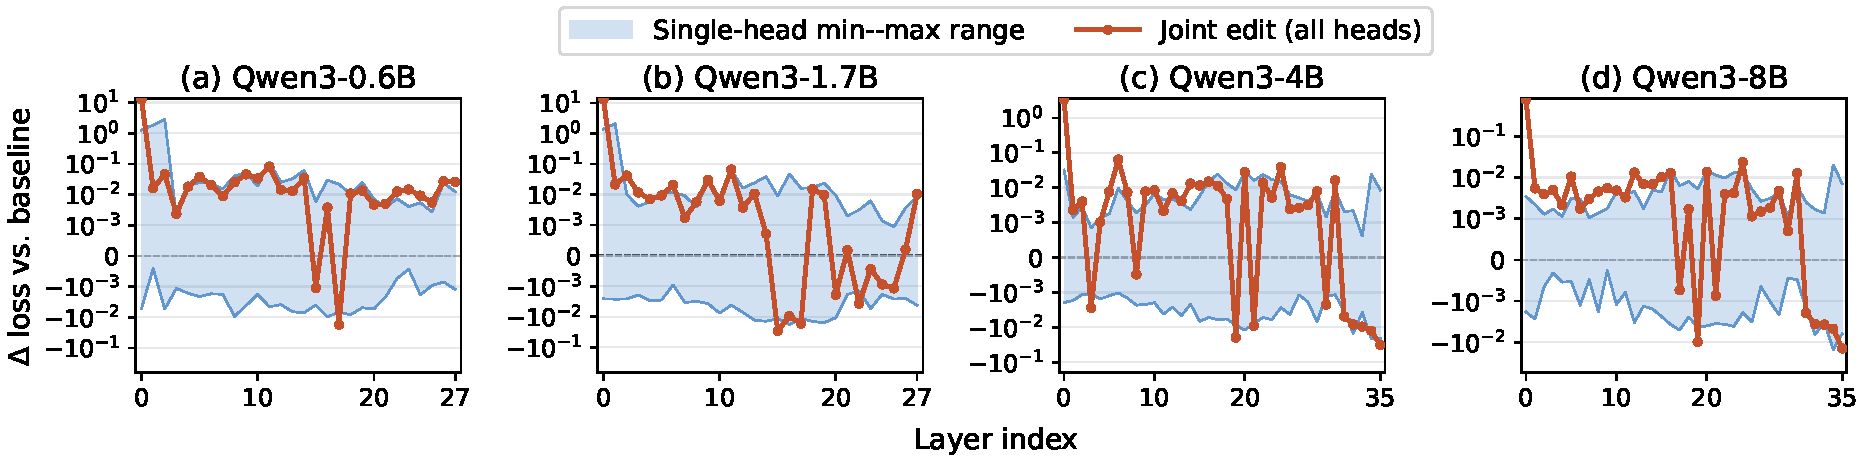
\includegraphics[
        width=0.245\textwidth,
        trim=307bp 0bp 0bp 218bp,
        clip
      ]{figs/per_head_causal_sensitivity_fullrem/head_delta_loss.pdf}%
    }
  \fi
  \caption{\textbf{All-layer head sensitivity across Qwen3 scales.}
  At each layer, orange shows joint full removal from all heads and the blue
  band spans the minimum and maximum isolated single-head effects; it is not a
  confidence interval. $\Delta$ loss is edited minus baseline over 128 fixed C4
  texts (positive is worse), shown on symmetric-log axes.}
  \label{fig:per-head-causal-sensitivity}
\end{figure*}

\section{MLP-Internal Geometry}
\label{app:mlp-internal-carrier}

Residual-space editing observes only the final MLP output, so it does not
show whether the same directional asymmetry is already present before the
down projection. Inside a gated MLP, the post-gating carrier and down-projected output are
\begin{equation}
  \begin{aligned}
    h &= \phi(W_{\mathrm{gate}}x)\odot W_{\mathrm{up}}x, \\
    y &= \sum_g y_g, \\
    y_g &= W_{\mathrm{down}}[:,I_g]h_g,
  \end{aligned}
  \label{eq:mlp-internal-sites}
\end{equation}
where $h_g=h[I_g]$. We choose residual-width groups, so $h_g$, $y_g$,
and $x$ have the same dimensionality. This exposes two internal editing
sites: each carrier $h_g$ is decomposed relative to $x$ before the down
projection, and each projected contribution $y_g$ is decomposed relative to
its carrier $h_g$ before the group contributions are summed. These controls
distinguish geometry already present in the gated intermediate representation
from geometry introduced by the down projection.
Table~\ref{tab:mlp-internal-carrier} reports fixed-token loss on Qwen3-0.6B.
At the two internal sites, full parallel removal changes loss by at most 0.0301,
whereas perpendicular removal increases it by more than 13 points.

\begin{table}[!htbp]
  \centering
  \small
  \caption{\textbf{MLP-internal component removal.}
  Values are edited-minus-no-op loss on fixed C4 tokens (lower is better).
  Full No-Para or No-Perp sets the named retained scale to zero; every no-op
  matches baseline.}
  \label{tab:mlp-internal-carrier}
  \resizebox{\columnwidth}{!}{%
  \begin{tabular}{lrr}
    \toprule
    Geometry & Full No-Para & Full No-Perp \\
    \midrule
    Residual MLP ($y$ relative to $x$) & +0.1165 & +15.9567 \\
    Grouped $h$ relative to $x$ & +0.0301 & +13.4184 \\
    Grouped $y_g$ relative to $h_g$ & \textbf{+0.0037} & +13.3324 \\
    \bottomrule
  \end{tabular}}
\end{table}

Table~\ref{tab:mlp-internal-downstream} reports matched downstream controls
beyond fixed-token loss.

\begin{table}[!t]
  \centering
  \scriptsize
  \caption{\textbf{Downstream controls for MLP-internal geometry.}
  Core-MC averages nine 0-shot benchmarks; MMLU is 5-shot. GSM8K-S/F are
  strict/flexible exact match, TQA R-L is TruthfulQA-generation Rouge-L, and
  DROP/CoQA use F1.}
  \label{tab:mlp-internal-downstream}
  \begin{minipage}[t]{\linewidth}
  \centering
  \textbf{(a) Multiple-choice controls}\par\smallskip
  \setlength{\tabcolsep}{3pt}
  \resizebox{\linewidth}{!}{%
  \begin{tabular}{llrr}
    \toprule
    Model & Setting & Core-MC & MMLU \\
    \midrule
    Qwen3-0.6B & Baseline & 50.94 & 52.40 \\
    & Full No-Para & 50.98 & 52.66 \\
    & Full No-Perp & 36.62 & 26.89 \\
    \midrule
    Qwen3-1.7B & Baseline & 55.19 & 60.21 \\
    & Full No-Para & 55.28 & 60.39 \\
    & Full No-Perp & 37.35 & 24.40 \\
    \bottomrule
  \end{tabular}}
  \end{minipage}\par\medskip
  \begin{minipage}[t]{\linewidth}
  \centering
  \textbf{(b) Generation and question-answering controls}\par\smallskip
  \setlength{\tabcolsep}{2pt}
  \renewcommand{\arraystretch}{1.37}
  \resizebox{\linewidth}{!}{%
  \begin{tabular}{@{}llrrrrr@{}}
    \toprule
    Model & Setting & GSM8K-S & GSM8K-F & TQA R-L & DROP & CoQA \\
    \midrule
    Qwen3-0.6B & Baseline & 49.43 & 50.42 & 18.98 & 7.76 & 74.24 \\
    & Full No-Para & 49.96 & 50.72 & 15.61 & 7.66 & 74.04 \\
    \midrule
    Qwen3-1.7B & Baseline & 68.76 & 68.92 & 48.34 & 7.32 & 77.06 \\
    & Full No-Para & 68.08 & 68.01 & 48.32 & 7.44 & 77.69 \\
    \addlinespace[1.6pt]
    \bottomrule
  \end{tabular}}
  \end{minipage}
\end{table}

\section{Pretraining Configuration Details}
\label{app:training-configs}

\begin{table*}[!t]
  \caption{\textbf{Task-wise post-training benchmark scores.}
  Avg. is unweighted and \(\Delta\)Avg uses the same-scale baseline. Base,
  Attn, and V-Para denote baseline, residual-space attention parallel removal,
  and full-aggregate value-space parallel removal.}
  \label{tab:appendix-pretraining-downstream}
  \centering
  \small
  \setlength{\tabcolsep}{4pt}
  \begin{tabular}{@{}llrrrrrrrr@{}}
    \toprule
    Model & Setting & ARC-E & BoolQ & HSwag & OBQA & PIQA & WinoGr & Avg & $\Delta$Avg \\
    \midrule
    \multirow{3}{*}{1.4B}
      & Base & 56.0 & \textbf{65.1} & 60.5 & 34.7 & 75.8 & 58.7 & 58.5 & 0.0 \\
      & Attn & 57.1 & 63.9 & 61.3 & 35.3 & 76.0 & 59.1 & 58.8 & +0.3 \\
      & V-Para & \textbf{58.3} & 62.8 & \textbf{62.1} & \textbf{35.9} & \textbf{76.3} & \textbf{59.8} & \textbf{59.2} & \textbf{+0.7} \\
    \midrule
    \multirow{3}{*}{2.7B}
      & Base & 58.4 & 61.2 & 66.0 & 37.1 & 76.5 & 61.8 & 60.2 & 0.0 \\
      & Attn & 59.3 & 62.8 & 66.7 & 37.7 & 77.0 & 62.1 & 60.9 & +0.7 \\
      & V-Para & \textbf{60.4} & \textbf{64.4} & \textbf{67.1} & \textbf{38.2} & \textbf{77.6} & \textbf{62.6} & \textbf{61.7} & \textbf{+1.5} \\
    \bottomrule
  \end{tabular}
  \vspace{0.5em}
\end{table*}

Table~\ref{tab:appendix-pretraining-downstream} resolves the summary averages
into task-level scores.
The trajectories in Figure~\ref{fig:pretraining} use OpenWebText, and the
1.4B/2.7B runs use FineWeb100BT from FineWeb~\citep{penedo2024the}. In every
setting, the full-aggregate value-space intervention is applied at every
layer.

The OpenWebText configurations labeled 296M, 436M, and 528M use
(layers, heads, width) of $(14,16,1024)$, $(16,18,1152)$, and
$(18,20,1280)$; the 1.4B and 2.7B configurations use $(24,16,2048)$ and
$(32,20,2560)$. The larger runs use eight DDP processes, approximately 104.9B
tokens, 2,048-token contexts, 200K updates, and global batch 256. For the 1.4B
model, the per-process micro-batch is 2, the
accumulation factor is 128, and the peak/minimum learning rates are
$4\times10^{-4}/4\times10^{-5}$; the corresponding settings for the 2.7B model
are 1, 256, and $3\times10^{-4}/3\times10^{-5}$. Shared settings are a 2K-step
warm-up with cosine decay, AdamW $\beta=(0.9,0.95)$, weight decay 0.1, gradient
clipping at 1.0, no dropout, seed 1337, and 200-batch evaluation every 1K
updates.

\noindent\begin{minipage}{\linewidth}
\paragraph{Gated parallel-scaling diagnostic.}
Figure~\ref{fig:appendix-1p4-trainable-scale} compares baseline, fixed V-Para
Rem., and gated parallel-scaling in the 1.4B run. Fixed removal has the lowest
training-loss trajectory among the three settings.
\end{minipage}

\begin{figure}[!htbp]
  \centering
  
\includegraphics[width=\linewidth]{figs/loss_curves/loss_1p4_gate_vs_xsa_absolute.pdf}
  \caption{\textbf{Parallel-scale adjustment during 1.4B pretraining.}
  FineWeb100BT training loss (lower is better) is plotted against
  update. Fixed V-Para sets the full-aggregate $s_{\parallel}=0$;
  trainable scaling instead predicts a tokenwise parallel scale.}
  \label{fig:appendix-1p4-trainable-scale}
\end{figure}

\section{Extended Compression Geometry}
\label{app:compression}

We use the normalization from Figure~\ref{fig:local-flip-attn}.
Figure~\ref{fig:appendix-compression-breakdown} extends the breakdown to the
accumulated update and the MLP output, and
Table~\ref{tab:local-total-perp-alignment} reports the layerwise correlation
between total and perpendicular attention-output error.

\begin{table}[H]
  \centering
  \scriptsize
  \setlength{\tabcolsep}{3.5pt}
  \caption{\textbf{Attention-output total error is mostly aligned with
  perpendicular error.}
  On Qwen3-4B and 12 fixed prompts, $r$ and $\rho$ are layerwise Pearson and
  Spearman correlations between normalized total error
  \(\|e\|/\|\Delta_{\mathrm{base}}\|\) and its perpendicular or parallel
  component. Perp./Total and Para./Total are mean component-to-total ratios
  across layers.}
  \label{tab:local-total-perp-alignment}
  \setlength{\tabcolsep}{3.3pt}
  \begin{tabular}{lccccc}
    \toprule
    Setting & \(r(e,e_{\perp})\) & \(\rho(e,e_{\perp})\) &
    \(\rho(e,e_{\parallel})\) & Perp./Total & Para./Total \\
    \midrule
    Quantization & \textbf{0.998} & \textbf{0.990} & 0.596 & \textbf{0.980} & 0.168 \\
    Unstructured & 0.970 & 0.909 & \textbf{0.810} & 0.891 & \textbf{0.439} \\
    4:8 & 0.986 & 0.986 & -0.135 & 0.887 & 0.415 \\
    2:4 & 0.991 & 0.979 & -0.432 & 0.875 & 0.425 \\
    \bottomrule
  \end{tabular}
\end{table}

\begin{figure*}[!t]
  \centering
  \begin{subfigure}[t]{0.485\textwidth}
    \centering
    
\includegraphics[width=\linewidth]{figs/comp_analysis/local_flip_compare-block_out-perp_over_base_update.pdf}
    \vspace{-0.35em}
    
\includegraphics[width=\linewidth]{figs/comp_analysis/local_flip_compare-mlp_out-perp_over_base_update.pdf}
    \caption{Perpendicular-error breakdown.}
    \label{fig:appendix-compression-perp}
  \end{subfigure}
  \hfill
  \begin{subfigure}[t]{0.485\textwidth}
    \centering
    
\includegraphics[width=\linewidth]{figs/comp_analysis/local_flip_compare-block_out-para_over_base_update.pdf}
    \vspace{-0.35em}
    
\includegraphics[width=\linewidth]{figs/comp_analysis/local_flip_compare-mlp_out-para_over_base_update.pdf}
    \caption{Parallel-error breakdown.}
    \label{fig:appendix-compression-para}
  \end{subfigure}
  \caption{\textbf{Compression-geometry breakdown across branches.}
  The left and right groups show perpendicular and parallel error,
  respectively. Within each group, the upper and lower panels show
  compressed-minus-baseline error for the accumulated attention-plus-MLP
  update and the MLP output, each normalized by the full baseline-update norm.
  Curves are layerwise means, with bands showing one standard deviation over 12 fixed prompts on
  Qwen3-4B. Settings are 4-bit AWQ and 50\% Wanda pruning with
  unstructured, 4:8, or 2:4 masks.}
  \label{fig:appendix-compression-breakdown}
  \vspace{8pt}
\end{figure*}

\begin{samepage}
\paragraph{Connecting Layer Dropping and Representation Evolution.}
The parallel/perpendicular view also decomposes a cosine-based diagnostic used
for layer dropping
\citep{He2026UncoveringTR}.
Let \(x\) be the incoming representation and let a layer update decompose as
\(\Delta=\Delta_{\parallel}+\Delta_{\perp}\), with
\(\Delta_{\parallel}=\alpha x\) and
\(\|\Delta_{\perp}\|=\beta\|x\|\). Then
\[
  \cos(x,x+\Delta)=
  \frac{1+\alpha}{\sqrt{(1+\alpha)^2+\beta^2}}.
\]
\end{samepage}%
The diagnostic depends on \(|\beta/(1+\alpha)|\). In the positive-scale,
small-angle regime,
\(1-\cos(x,x+\Delta)\approx
\frac{1}{2}\left(\beta/(1+\alpha)\right)^2\).
Figure~\ref{fig:baseline-update-over-hidden} reports the baseline update
magnitudes.

\begin{figure*}[!b]
  \centering
  
\includegraphics[width=0.65\textwidth]{figs/comp_analysis/baseline_update_over_hidden_state.pdf}
  \caption{\textbf{Baseline layer updates are small relative to the
  residual stream.} Means and one-standard-deviation bands for
  \(\|\Delta_{\mathrm{base}}\|/\|x\|\) across 12 prompts for Qwen3-4B layers
  1--34, shown for the accumulated attention-plus-MLP update, attention
  output, and MLP output. Values below one indicate updates smaller than the
  incoming residual stream.}
  \label{fig:baseline-update-over-hidden}
  \vspace{1em}
\end{figure*}
